\section{Results}
\label{sec:results}

\subsection{AI model cards}

The level of documentation varies greatly from model to model. We have set up an
automatic documentation system for models trained within \Gls{WIPP}.

\subsection{WIPP 2-steps workflow}

The WIPP 2-steps workflow is first, do the inference of the model and then
compute the accuracy.

\begin{figure}[H]
  \centering
  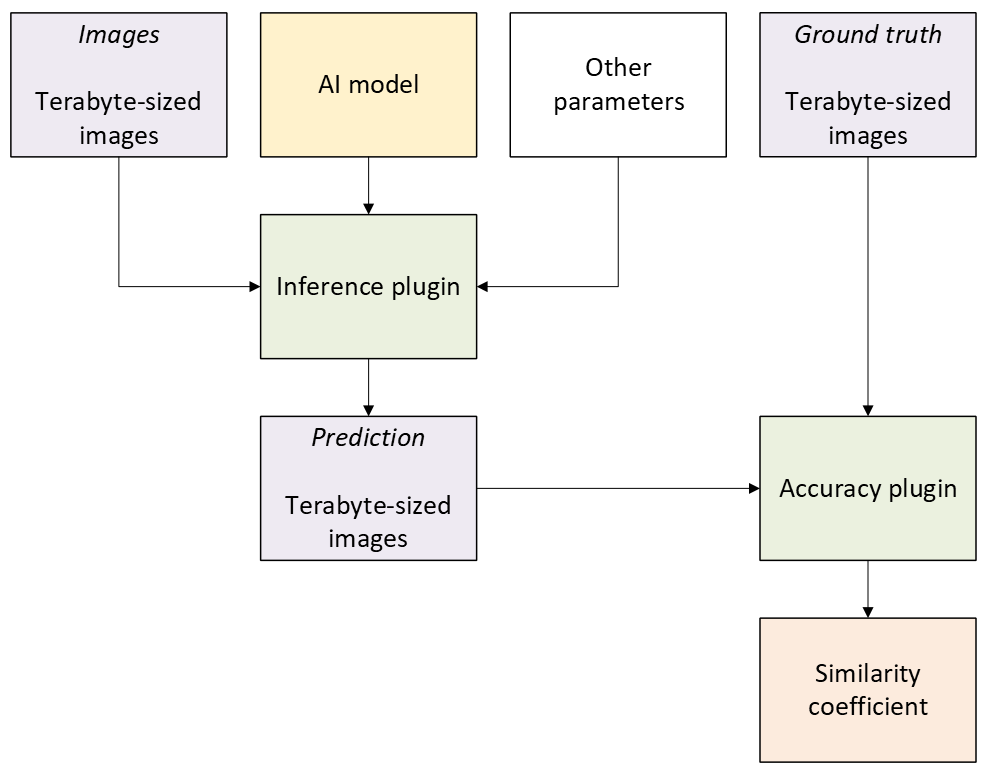
\includegraphics[width=1.0\linewidth]{png/results/workflow.png}
  \caption{WIPP 2-steps workflow}
  \label{fig:workflow}
\end{figure}

We compute everything in \Gls{WIPP}. The \Gls{WIPP} server specifications are:
\begin{itemize}
  \item CPU: AMD Ryzen 9 3950X 16-Core Processor with 2 threads
  \item GPU: NVIDIA GeForce RTX 3090
  \item 64G RAM
\end{itemize}

\subsection{Dataset 'cell boundary'}

We use the 'Retinal Pigment Epithelium' dataset. There are 1032 images of type
'cell microscopy' with size 256$\times$256.

\medskip

\begin{minipage}[h!]{0.20\textwidth}
  \centering
  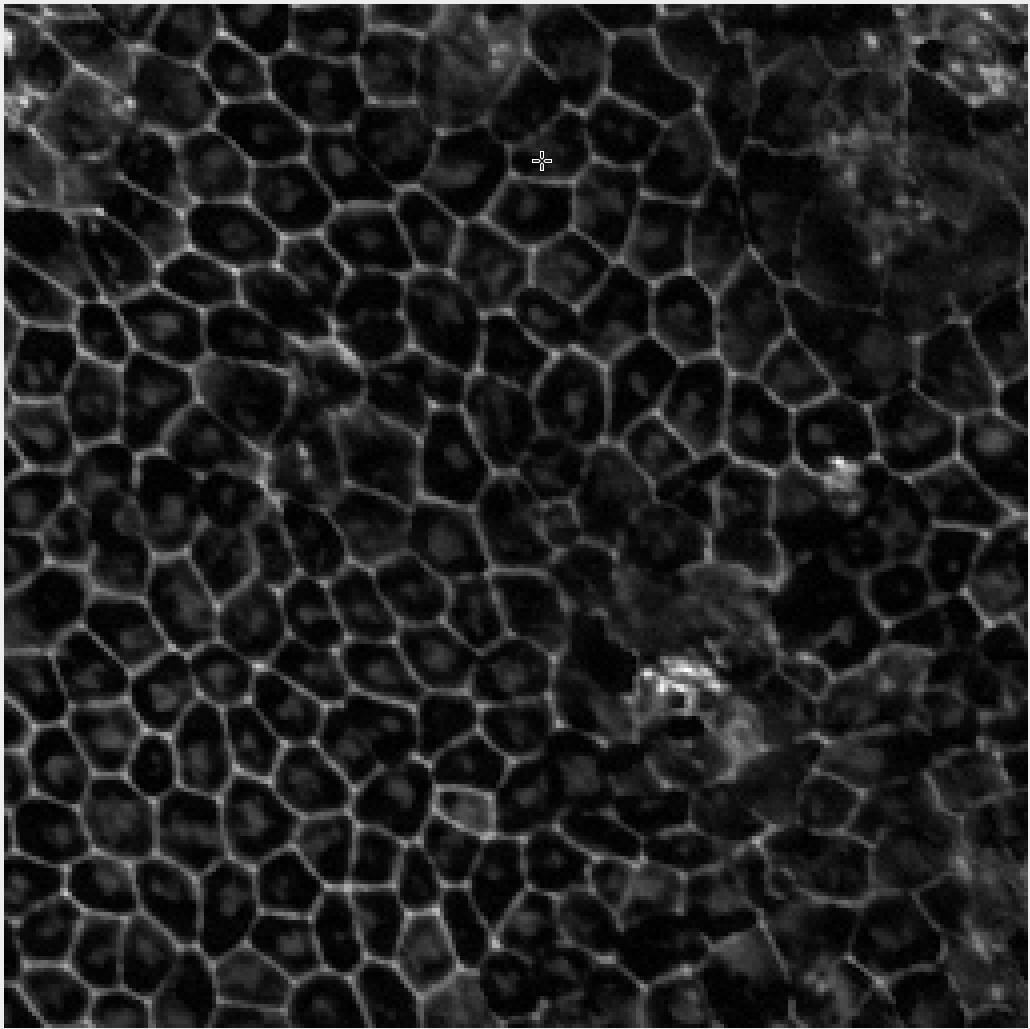
\includegraphics[scale=0.1]{./png/results/cell_image.png}
  \textbf{Image}
\end{minipage}\hfill
\begin{minipage}[h!]{0.20\textwidth}
  \centering
  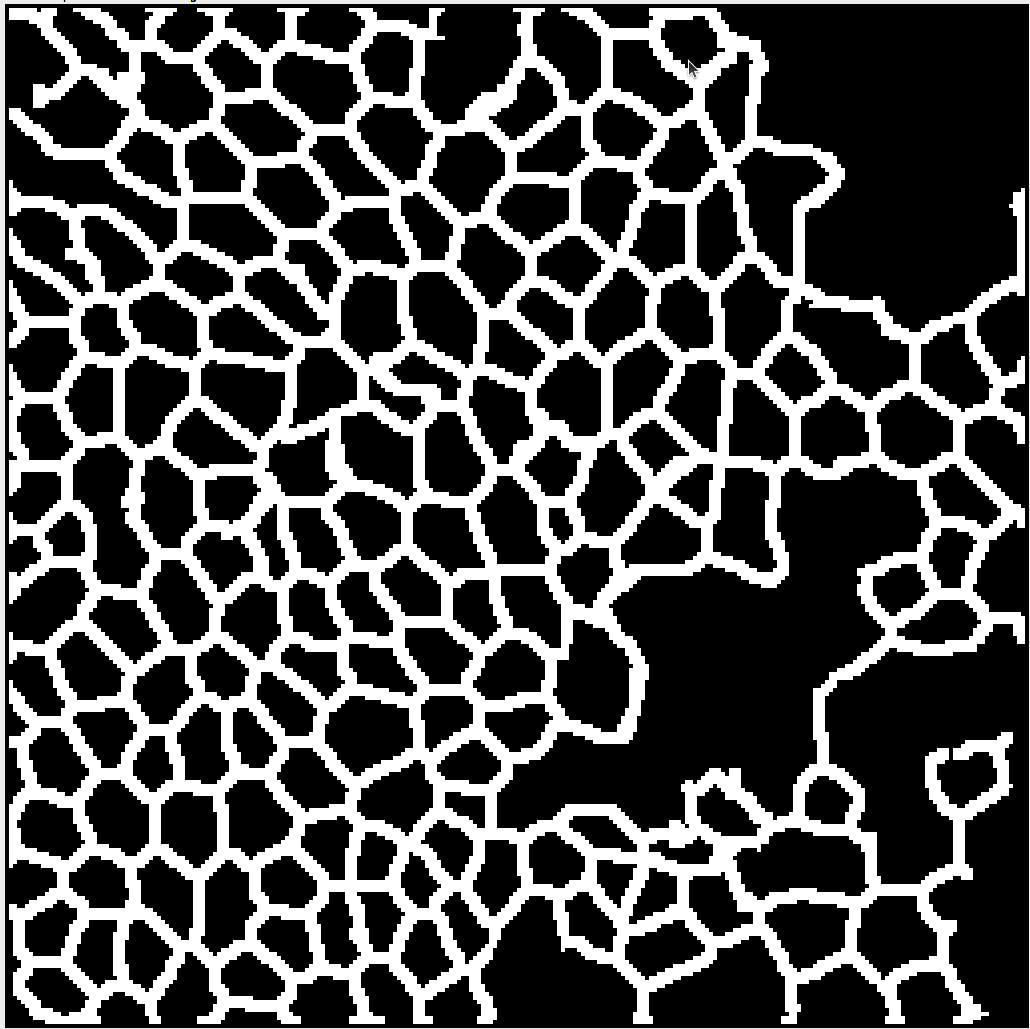
\includegraphics[scale=0.1]{./png/results/cell_mask.png}
  \textbf{Mask}
\end{minipage}

\medskip

Source: https://doi.org/doi:10.18434/T4/1503229

\subsection{Benchmark 'cell boundary'}

We inference different models to do the 'segments cell edges' task.

\begin{table}[H]
  \footnotesize
  \centering
  \caption{Accuracy after inference on data 'cell boundary'}
  \begin{tabular}{llcc}
    \toprule
    Repository    & Model                       & Accuracy             \\ [0.5ex]
    \midrule
    WIPP          & unet-cnn*                   & 95.11\% $\pm$ 0.78\% \\
    BioImage.IO   & 10.5281/zenodo.5869899      & 89.30\% $\pm$ 0.84\% \\
    Hugging Face  & facebook/sam-vit-huge       & 86.01\% $\pm$ 2.50\% \\
    SAM2          & facebook/sam2.1-hiera-large & 80.18\% $\pm$ 5.02\% \\
    Cellpose      & cyto3                       & 78.51\% $\pm$ 2.35\% \\
    \bottomrule
  \end{tabular}
  \caption*{*Trained then inferenced in WIPP}
\end{table}

\subsection{Dataset 'nuclei segmentation'}

We use the 'Kaggle 2018 Data Science Bowl' dataset. There are 497 images of type
'cell microscopy' with size 256$\times$256 and 696$\times$520.

\medskip

\begin{minipage}[h!]{0.20\textwidth}
  \centering
  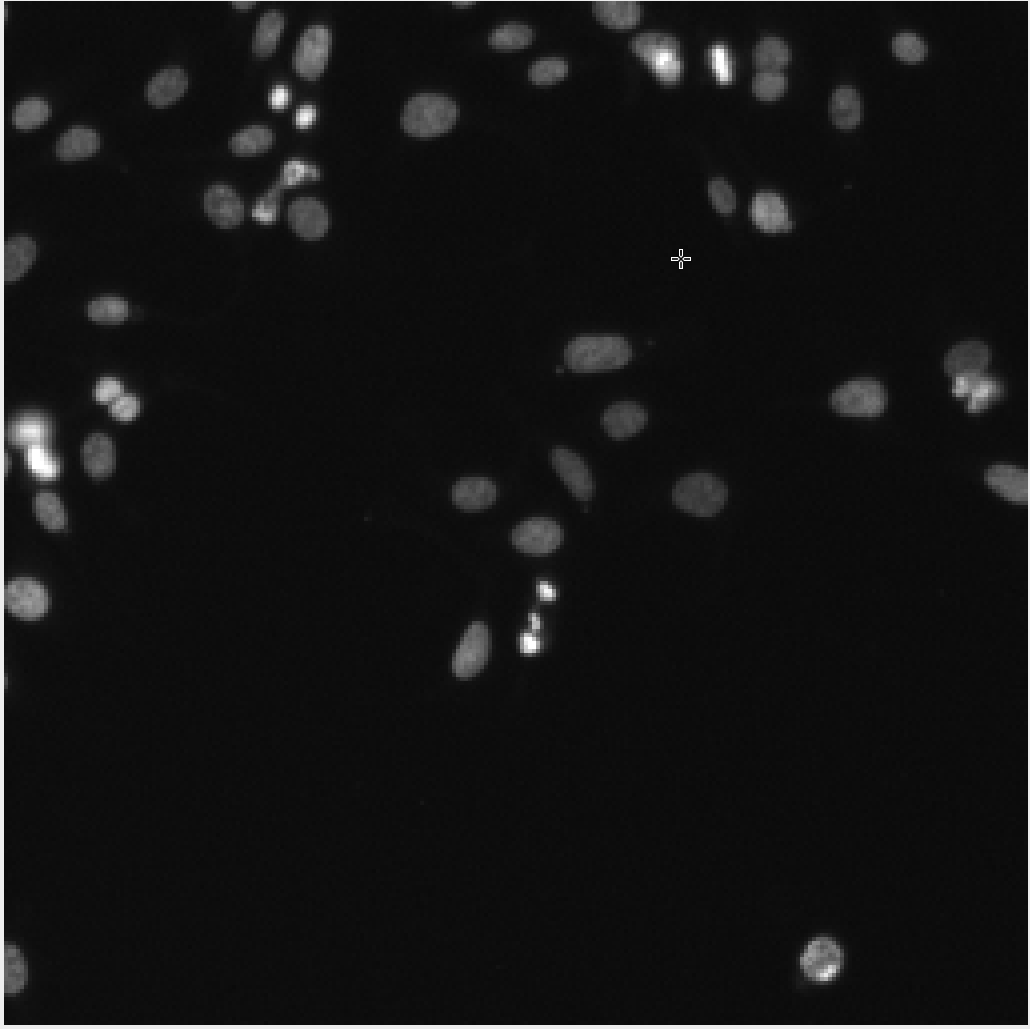
\includegraphics[scale=0.1]{./png/results/nuclei_image.png}
  \textbf{Image}
\end{minipage}\hfill
\begin{minipage}[h!]{0.20\textwidth}
  \centering
  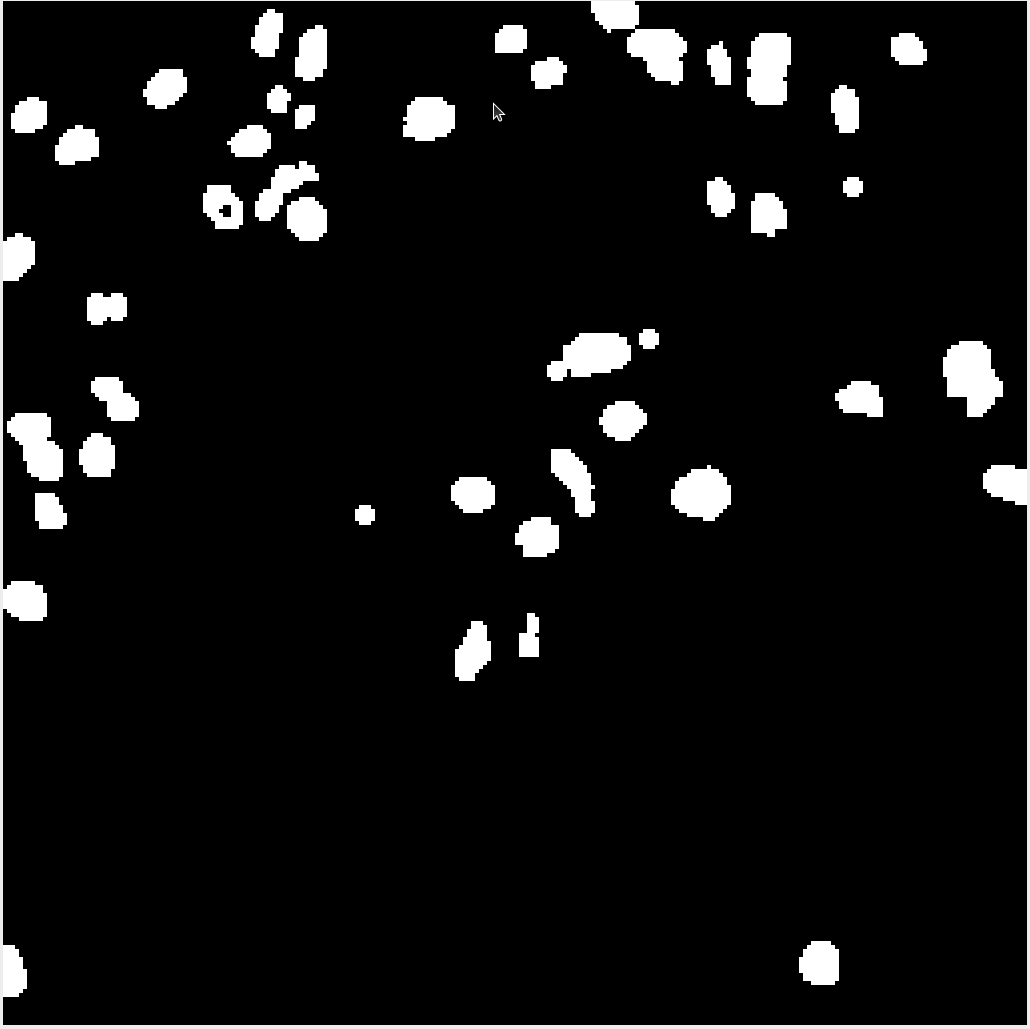
\includegraphics[scale=0.1]{./png/results/nuclei_mask.png}
  \textbf{Mask}
\end{minipage}

\medskip

Source: https://bbbc.broadinstitute.org/BBBC038/

\subsection{Benchmark 'nuclei segmentation'}

We inference different models to do the 'segments nuclei of cells' task.

\begin{table}[H]
  \footnotesize
  \centering
  \caption{Accuracy after inference on data 'nuclei segmentation'}
  \begin{tabular}{llcc}
    \toprule
    Repository    & Model                       & Accuracy               \\ [0.5ex]
    \midrule
    BioImage.IO  & 10.5281/zenodo.5764892        & 93.73\% $\pm$ 3.98\%  \\
    WIPP         & Stardist 2D paper DSB 2018*   & 90.67\% $\pm$ 4.42\%  \\
    Cellpose     & cyto3                         & 82.31\% $\pm$ 17.25\% \\
    Cellpose     & nuclei                        & 81.00\% $\pm$ 21.00\% \\
    SAM2         & facebook/sam2.1-hiera-small   & 48.18\% $\pm$ 32.41\% \\
    SAM2         & facebook/sam2.1-hiera-large   & 33.89\% $\pm$ 29.43\% \\
    BioImage.IO  & 10.5281/zenodo.5869899        & 29.47\% $\pm$ 8.32\%  \\
    Hugging Face & facebook/sam-vit-huge         & 21.63\% $\pm$ 15.37\% \\
    \bottomrule
  \end{tabular}
  \caption*{*Trained then inferenced in WIPP}
\end{table}

\subsection{Notes}

Even if the results may not be perfect, this method allows you to quickly try
out a new model at reduced cost. It is also easy to change dataset. We hope to
improve the speed of data analysis and enable better overall results.
